Den anden metode man kan bruge kaldes for et dynamisk Huffman træ. Et dynamisk træ bliver genereret ud fra den reelle data, som teksten består af. Træet bliver genereret ud fra den specifikke besked, og er ikke en generel liste som ved den statiske metode. Det dynamiske træ er derfor det mest optimale træ til Huffman coding. Den dynamiske opbygning af et træ starter med at sætte de to tegn med færrest forekomster sammen til en knude. Derefter bliver den knude sat sammen med det næste tegn, som forekommer mindst og er endnu ikke sat ind i træet, og sat til en ny knude. Denne process fortsættes indtil alle tegn er blevet sat ind i træet, og der er en rod i toppen af træet. Figur \ref{fig:dynamic_tree} viser dette.

\begin{figure}[H]
\centering
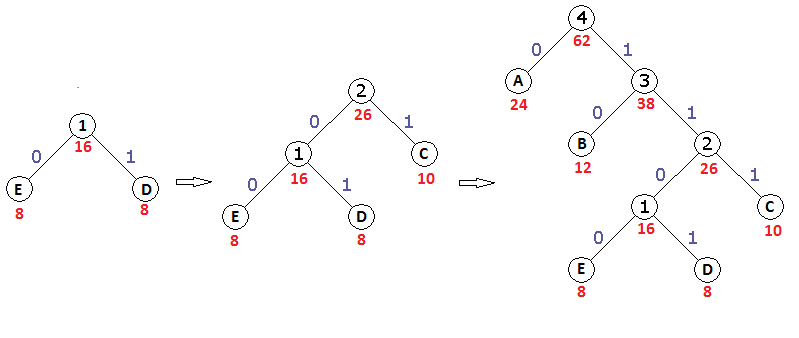
\includegraphics[width=\linewidth]{Billeder/dynamisk.png}
\caption{Dynamisk opbygning af et Huffman træ udfra det tidligere eksempel \cite{Hufftree_1}}
\label{fig:dynamic_tree}
\end{figure}

En ulempe ved den dynamiske metode er, at for at kunne dekode den komprimeret tekst skal man bruge en kode tabel over træet. Idet at det er et træ skræddersyet til et bestemt stykke tekst, så har dem der skal dekode teksten ingen mulighed for at oversætte 0 og 1 tallene tilbage til den oprindelige tekst. Derfor er det nødvendigt, med den dynamiske metode, at medsende en tabel som angiver hvilke tegn der har hvilke bitmønstre. Dette betyder selvfølgelig, at den komprimerede tekst fylder et stykke mere, og gør derfor ikke optimalt brug af komprimeringskraften ved Huffman coding. \cite{Hufftree_4}

Fordelen ved et dynamisk træ i forhold til det statiske er, at den mere konstant gør optimal brug af Huffman coding til at komprimere et stykke tekst. Det er selvfølgelig det man gerne vil opnå i forhold til SMS beskeder, men som sagt så er det nødvendigt at sende en tabel med, så det er muligt at dekode den komprimerede tekst. Dette betyder at SMS beskeden fylder mere end hvis det bare var det komprimerede stykke tekst, og arbejder derfor imod målet om at formindske størrelsen, af den data der bliver sendt.